\section{\label{section:ExecutiveComponents}Executive Components}

The GMAT executive subsystem is built around four classes: the Moderator, the Configuration
Manager, the Sandbox, and the Publisher.  Each of these classes is a singleton in the GMAT
executable.

\subsection{Moderator}



\subsection{Configuration Manager}



\subsection{\label{section:Sandbox}The Sandbox}


\subsubsection{\label{section:SandboxCloning}Configured Object Cloning}


\subsubsection{\label{section:SandboxLateBinding}The Late Binding Strategy}


\subsection{Publisher}



\subsection{Executive Component Interactions}



\section{\label{section:InterfaceOverview}Interface Components}

% The interfaces to GMAT can be broken into interfaces with external system and interfaces with
% users.  The external interface component is used to provide an interface between GMAT and MATLAB.
% Other external systems may be interfaces to GMAT in future builds.  The internal interfaces are
% used to let the user control GMAT, either through custom text files called scripts, or through
% direct manipulation to objects managed in GMAT.  Figure~\ref{InterfacePackages} shows the
% main classes used to implement these interfaces.  The two major subdivisions are outlined here.
% Details of the design for these components can be found in chapters~\ref{chapter:ScriptRW},
% \ref{chapter:TheGui}, and \ref{chapter:ExternalInterfaces}.

%\begin{figure}[htb]
%\begin{center}
%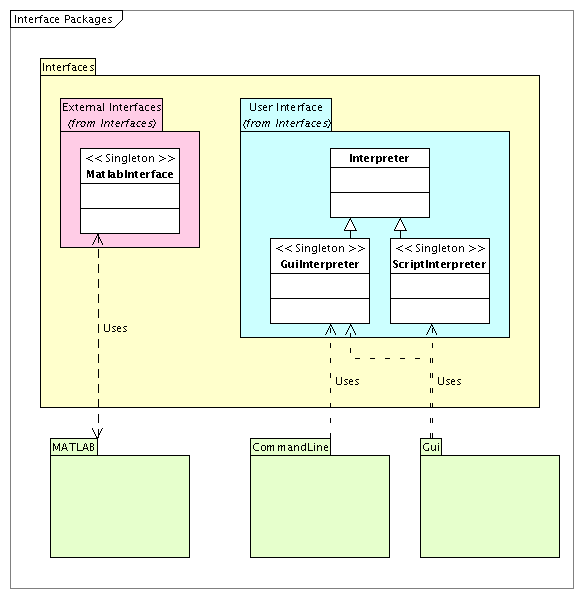
\includegraphics[420,430]{Images/InterfacePackages.png}
%\caption{\label{InterfacePackages}Interface Packages}
%\end{center}
%\end{figure}

\subsection{User Interfaces}

GMAT can be run from either a command line interface or a graphical user interface (GUI).  These
interfaces are connected to the core GMAT code through objects in the User Interface
portion of the Interface subsystem. The command line interface controls GMAT exclusively through
the singleton ScriptInterpreter  The GUI uses the ScriptInterpreter to read and write GMAT files
and to preview GMAT scripts, and the GuiInterpreter for other interactions with the internal GMAT
objects.

The command line interface provides minimal feedback during a run.  Users can use the command line
interface to execute GMAT scripts, either one at a time or in a batch mode.  The interface displays
status messages during the run, but provides no other feedback regarding the status of a script
run.  In batch mode, the interface runs multiple scripts sequentially based on the input from a
batch file.  Statistics regarding the success or failure of the individual scripts are collected
and displayed at the end of the run.

The graphical user interface is implemented using the wxWidgets GUI Library \cite{wxWidgets}.
It provides a rich development environment for the implementation of the user interface.  The GMAT
GUI is built on all three target platforms (Windows XP, MacIntosh OS X, and Linux) using the same
GUI code, with minimal customization for the different platforms.  The communications layer between
this library and core GMAT functionality is the GuiInterpreter.  Further information about the GUI
can be found in Chapter~\ref{chapter:TheGui}.

All scripting capabilities in GMAT are implemented using the ScriptInterpreter and its helper
classes.  This component is discussed in Chapter~\ref{chapter:ScriptRW}.  The GMAT scripting
language is documented in the \textbf{GMAT Mathematical Specifications and User's Guide}
\cite{mathSpec}, a companion volume to this document.

\subsection{External Interfaces}



\section{\label{section:ModelOverview}Model Elements}



\section{\label{section:FactoryOverview}Factories}



\section{\label{section:Namespaces}Namespaces and Enumerations}

GMAT uses several namespaces defined for specific purposes.  The ``Gmat'' namespace is used to
define program specific enumerations defining the types of objects users can configure in GMAT, the
types of data structures commonly used in the system, and more specialized enumerations used by
some of GMAT's subsystems.

\subsection{Enumerations}

\subsubsection{The ObjectType Enumeration}

\begin{description}
\item[SPACECRAFT] This member is inityialized to the value 1001.
\item[FORMATION]
\item[SPACEOBJECT]
\item[GROUND\_STATION]
\item[BURN]
\item[COMMAND]
\item[PROPAGATOR]
\item[FORCE\_MODEL]
\item[PHYSICAL\_MODEL]
\item[TRANSIENT\_FORCE]
\item[INTERPOLATOR]
\item[SOLAR\_SYSTEM]
\item[SPACE\_POINT]
\item[CELESTIAL\_BODY]
\item[CALCULATED\_POINT]
\item[LIBRATION\_POINT]
\item[BARYCENTER]
\item[ATMOSPHERE]
\item[PARAMETER]
\item[STOP\_CONDITION]
\item[SOLVER]
\item[SUBSCRIBER]
\item[PROP\_SETUP]
\item[REF\_FRAME]
\item[FUNCTION]
\item[FUEL\_TANK]
\item[THRUSTER]
\item[HARDWARE] Tanks, Thrusters, Antennae, Sensors, etc.
\item[COORDINATE\_SYSTEM]
\item[AXIS\_SYSTEM]
\item[ATTITUDE]
\item[MATH\_NODE]
\item[MATH\_TREE]
\item[UNKNOWN\_OBJECT]
\end{description}

\subsubsection{The ParameterType Enumeration}

\begin{description}
\item[INTEGER\_TYPE]
\item[UNSIGNED\_INT\_TYPE]
\item[UNSIGNED\_INTARRAY\_TYPE]
\item[REAL\_TYPE]
\item[REAL\_ELEMENT\_TYPE]
\item[STRING\_TYPE]
\item[STRINGARRAY\_TYPE]
\item[BOOLEAN\_TYPE]
\item[RVECTOR\_TYPE]
\item[RMATRIX\_TYPE]
\item[TIME\_TYPE]
\item[OBJECT\_TYPE]
\item[OBJECTARRAY\_TYPE]
\item[ON\_OFF\_TYPE]
\item[TypeCount]
\item[UNKNOWN\_PARAMETER\_TYPE] = -1
\end{description}


\subsubsection{\label{section:WrapperDataTypeEnum}The WrapperDataType Enumeration}

Some components of GMAT need to access data elements in a generic fashion.  These components, most
notably including the Command subsystem, use a class of wrapper objects that take the disparate
types and present a common interface into those types.  The WrapperDataType enumeration is used to
identify the type of underlying object presented by the wrapper classes.  More information about
this object can be found in Section~\ref{section:DataWrappers}.

This enumeration has the following entries:

\begin{description}
\item[NUMBER] a Real or Integer value entered explicitly into the command.
\item[STRING] a text string with no associated object.
\item[OBJECT\_PROPERTY] an internal data member of an object, accessible using the GmatBase
parameter accessor methods (GetRealParameter(), GetIntegerParameter(), etc).
\item[VARIABLE] an instance of the Variable class.
\item[ARRAY] an instance of the Array class.
\item[ARRAY\_ELEMENT] an element of an Array object.
\item[PARAMETER\_OBJECT] any other object derived from the Parameter class.
\end{description}


\subsubsection{The RunState Enumeration}

\begin{description}
\item[IDLE] = 10000
\item[RUNNING]
\item[PAUSED]
\item[TARGETING]
\item[OPTIMIZING]
\item[SOLVING]
\item[WAITING]
\end{description}


\subsubsection{The WriteMode Enumeration}

\begin{description}
\item[SCRIPTING]
\item[SHOW\_SCRIPT]
\item[OWNED\_OBJECT]
\item[MATLAB\_STRUCT]
\item[EPHEM\_HEADER]
\end{description}


\subsection{Defined Data Types}

\begin{description}
\item[typedef std::vector<Gmat::ObjectType> ObjectTypeArray]
\end{description}
